

\section{Módszerek és megvalósítás}
\subsection{Eloszlásbecslés Bayesiánus formalizmussal}\label{sec:bayes}
Célunk az idegsejt modellezés eszközeivel adott mérési eredmények alapján különböző paraméterek poszterior eloszlását meghatározni a kiválasztott sejttípuson belül, mivel ez sok lényeges információt hordozhat (paraméterek várható értéke, közöttük levő korreláció, becslés információtartalma...). Erre a problémakörre jól alkalmazható a Baysiánus inferencia módszere, amit az alábbiakban tárgyalunk.

\paragraph{valószínűségi változók}
A modell paramétereire úgy tekintünk, mint valószínűségi változókra $(\xi)$, melyekhez eloszlásfüggvényt szeretnénk rendelni.

\paragraph{poszterior eloszlás}
Paraméterek poszterior eloszlását szeretnénk meghatározni adott kísérleti eredmények mellett.
Elsődleges szempont tehát, hogy legyenek kísérleti eredményeink $(D)$ (például a mi esetünkben passzív idegsejtek válasza áramimpulzus hatására). Valamint jellemezni kell valamilyen módon, hogy az adatok mennyire támasztják alá a modellünk adott paraméterek melletti helyességét $(\Lagr_i(D|\xi))$. Ezen kívül hasznos, ha vannak előzetes ismereteink a becsülendő paraméterekről $(\Pi(\xi))$, így kizárva azokat az eseteket, amelyek biztosan nem következhetnek be (pl. negatív értékeket nem vehetnek fel bizonyos biofizikai paraméterek). Ezen összetevőkből egy poszterior eloszlás készíthető a következő módon:

\begin{equation}\label{eq:bayes}
P(\xi|D) = \dfrac{\Lagr(D|\xi)\Pi(\xi)}{\int \Lagr(D|\xi)\Pi(\xi)d\xi}
\end{equation}

\begin{itemize}
	\item $P(\xi|D)$: Ez a poszterior eloszlás, a keresett paraméterek valószínűségi eloszlása a mérési adatok és az előzetes ismeretek figyelembevétele után.
	\item $\Lagr(D|\xi)$: Ez a likelihood eloszlás, azt jellemzi mennyire valószínű ezeknek az adatoknak a mérése, ha az adott paraméterbeállítással vett modellünket vesszük igaznak. A következő pontban ezt részletesen tárgyaljuk.
	\item $\Pi(\xi)$: Ez a prior eloszlás, előzetes ismereteink a paraméterekről. Úgy is felfoghatjuk, hogy ezt az eloszlást frissítjük az új adatok függvényében, így keletkezik a poszterior eloszlás. Új méréseket végezve ez a folyamat tovább iterálható.
	\item $\int \Lagr(D|\xi)\Pi(\xi)d\xi$: Ez csupán a normálási faktor. Annak a következménye, hogy a valószínűségi eloszlásoknak normáltnak kell lenniük, így teljes tartományra vett integráljuknak pedig egynek.
\end{itemize}

\paragraph{marginalizálás}
Előfordulhat, hogy néhány paraméterre ki szeretnénk marginalizálni az eloszlást, ezzel vizsgálva az egyes paraméterekre vett eloszlásokat, illetve a kiválasztott paraméterek együttes eloszlásait\footnote{Két paraméter együttes eloszlását még szépen meg lehet jeleníteni egy háromdimenziós ábrán, de efölött már nehézségekbe ütközünk.}. Tegyük fel, hogy $\xi$ a célparamétereink, de a modellt kiterjesztettük további $\theta$ változóval, amit viszont ki szeretnénk marginalizálni. Marginalizálás után a poszterior alakja ugyancsak $P(\xi|D)$ lesz.  A likelihood a kibővített paraméterekkel ilyen formában írható fel:
\[
\Lagr(D|\xi, \theta)
\]
A megcélzott változókat egyszerűen kiintegrálva (a priorjaival együtt) visszakapjuk a~\ref{eq:bayes}-es egyenletben szereplő likelihood formát:

\begin{eqnarray}\label{eq:marginalize}
\Lagr(D|\xi) = \int \Lagr(D|\xi, \theta)P(\theta)d\theta
\end{eqnarray}
Az így kapott a likelihood függvényben már csak a $\xi$ paraméterek szerepelnek változóként.

\paragraph{numerikus implementálás}
Numerikusan nem lehetséges egzaktul folytonos függvények kezelése. Mégis diszkrét eloszlások bevezetése helyett, \textit{kvázi-folytonosnak} tekintjük őket és alkalmazzuk rá a numerikus eljárásokat, mintha folytonosak lennének.




\subsection{Zajmodellek}\label{sec:noise}
A \ref{sec:bayes} fejezetben bevezettünk egy valószínűségi leírást, aminek fontos alkotóeleme a kísérleti adatsor $D$ -- mi esetünkben ez a passzív idegsejt áramimpulzusra adott feszültségválasza. Minden kísérletnél elkerülhetetlen tényező a zajok megjelenése. Tegyük fel, hogy van egy determinisztikus eredmény $(D^*)$, amire kísérleti zajt rakva $(z)$ kapjuk meg a valódi mért adatokat $(D)$. 
\[
D = D^* + z
\]
Fontos kiemelni, hogy ez tulajdonképpen a módszer alapfeltevése, miszerint a kísérletből kinyert adatsorunk úgy áll elő, mint egy determinisztikus függvényalak és az  arra rakódott zaj. Ez látható szemléletesen a \ref{fig:white} és \ref{fig:colored}-ábrákon.

Ez azt jelenti, ha jól ismerjük a kísérletből fakadó zajt, akkor szintetikus \textit{"kísérleti adatokat"} tudunk előállítani. Másrészt a zaj az inferencia lelke, mivel ez az egyik tényezője\footnote{A másik a modell érzékenysége a paraméterek megváltoztatására. Ha a paramétereket kicsit megpertulbálva nagyon elromlik a modell eredményessége, akkor pontosabb a becslés mintha a fordított eset állna elő.} a paraméterbecslés pontosságának, aminek a meghatározását tűztük ki célunkul. A likelihood függvénybe beleépítjük a zajmodellünket is, így paraméterbecslésnél -- amikor összevetjük a modellünk eredményét a kísérleti adatokkal -- tulajdonképpen a zajt is figyelembe vesszük, ami nagy előnye az eljárásnak a paraméteroptimalizációs megoldásokkal szemben.

Fontosabb minél realisztikusabb zajmodellel dolgozni, mivel az előállított szintetikus adatokon futtatva a paraméterbecslési módszerünk képesek leszünk előre megjósolni az egyes mérési összeállítások várható információtartalmát, majd összehasonlítva az eredményeket, a leghatékonyabbat kiválasztani a kísérletezőknek.

Kétfajta zajmodellel dolgoztunk: egy kezdetleges független zajjal, a fehér zajjal, valamint egy realisztikusabb, önmagával exponenciálisan korreláló (színes)\footnote{Konvenció szerint a független zajokat fehér zajoknak, az önmagával korreláló zajokat pedig színes zajoknak nevezzük. Elektrofiziológiai kísérleteknél tipikusan színes zajok jelennek meg.} zajjal. Ezekről lesz szó a következő pontokban, pontosabban arról, hogy hogyan is alkotjuk meg a zajmodellt, illetve mivel tudjuk jellemezni a zaj tulajdonságait.

\subsubsection{Autokorrelációs függvény}
A zajt jellemezhetjük autokorrelációs függvényével. Ez azt jellemzi, hogy a függvény mennyire hasonlít önmagára, azaz szemléletesen ha eltoljuk önmagán, mennyire fed át. Ha a mérőberendezéssel \textit{"üresjárásban"} mérünk (alapvonal), akkor tulajdonképpen a zajt mérjük. Ha megismételjük elegendően sokszor ezt a mérést és az adatokon elvégezzük az autokorrelációs vizsgálatot, majd átlagoljuk a kapott eredményeket, akkor meghatároztuk a zaj autokorrelációs függvényének alakját. Ez azt jellemzi, hogy a zaj mennyire korrelál önmagával időben. A \ref{fig:baseline}-ábrán látható sok \textit{"alapvonal"} felvétel. A \ref{fig:autocorrelation}-ábrán pedig ezeknek az autokorrelációja, illetve pirossal azok átlaga. Az ábrán szépen látszódik -- az átlagolt piros függvénymeneten -- az autokorrelációs függvények legfőbb jellemzője, mégpedig az hogy mindig $t=0$-ban van maximuma, hiszen ha a függvényt nem toljuk el, akkor tökéletesen korrelál (átfed) önmagával.

\begin{figure}[h!]
	\centering
	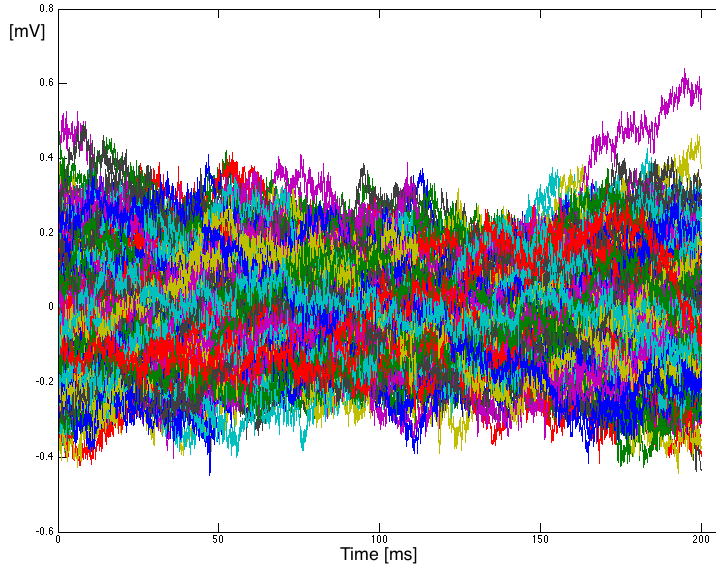
\includegraphics[width=0.7\linewidth]{fig/noise/bas2}
	\caption[Zaj baseline]{Sok \textit{"üresjárásban"} mért alapvonal (baseline) zajadat. Az egyes adatsorok különböző színnel jelölve.}
	\label{fig:baseline}
\end{figure}

\begin{figure}[h!]
	\centering
	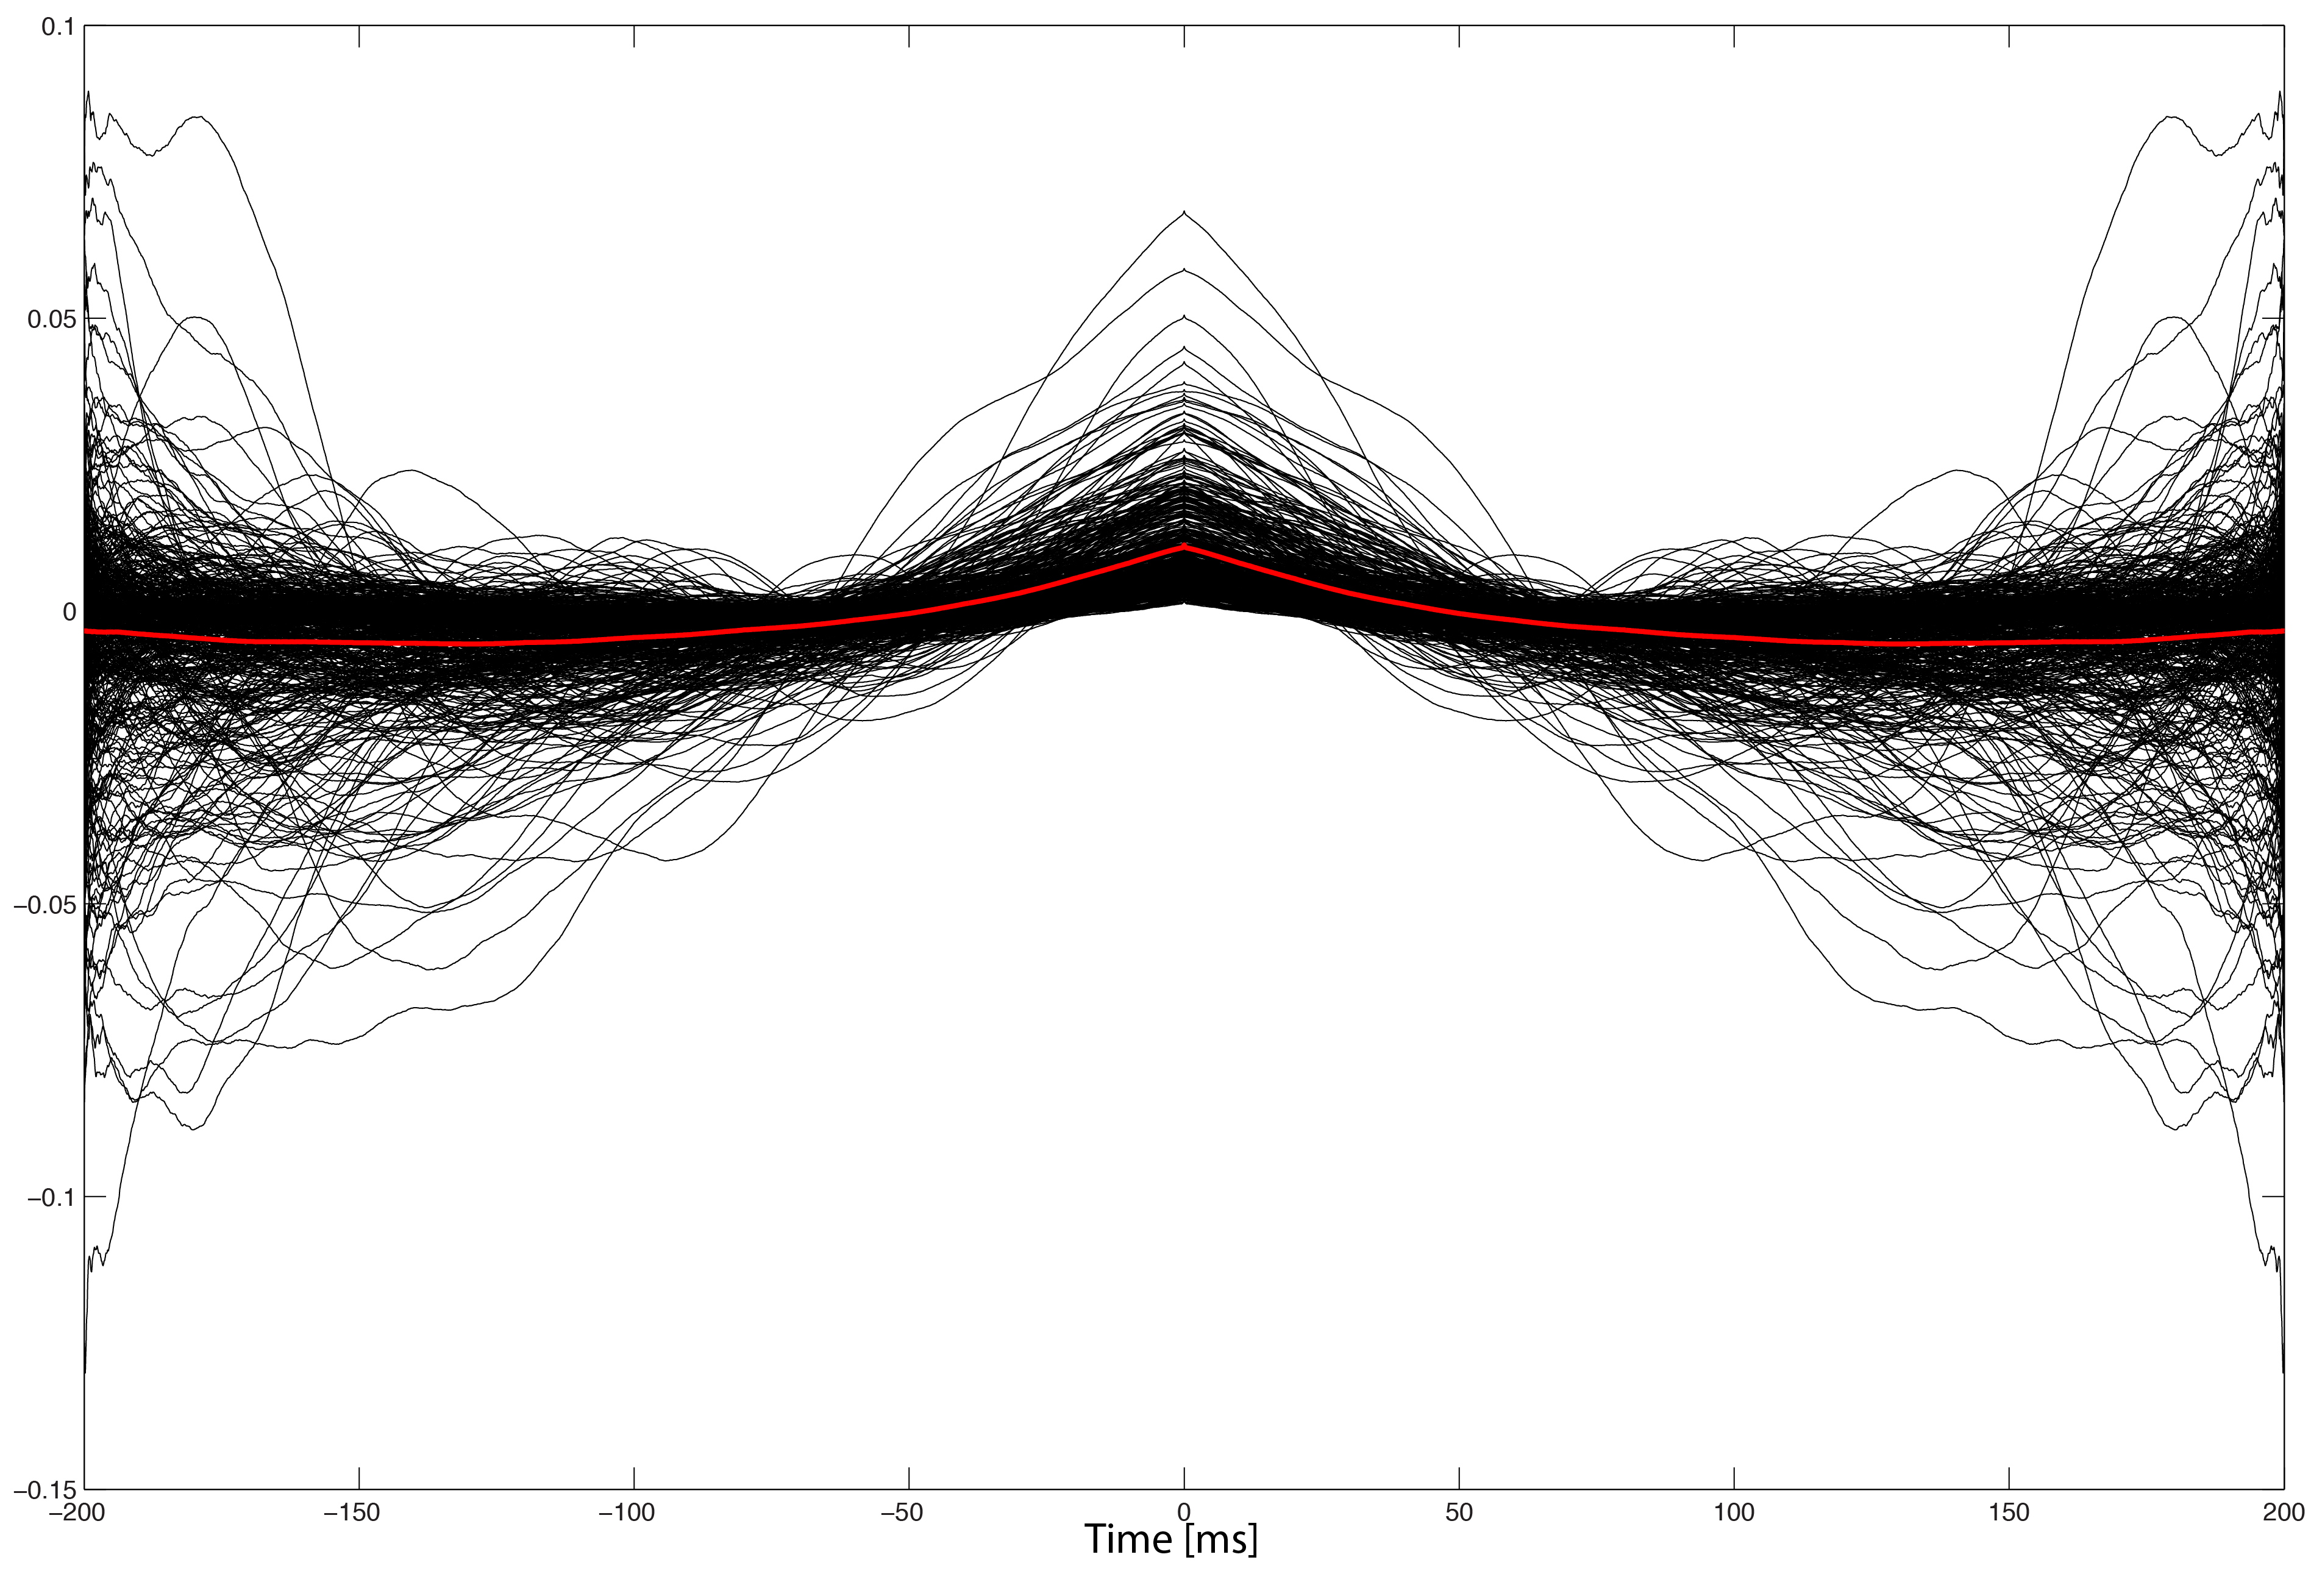
\includegraphics[width=0.8\linewidth]{fig/noise/autocorr.png}
	\caption[Zaj autokorrelációja]{Sok autokorrelációs eredmény feketével és azok átlaga pirossal. Exponenciális lecsengés jellegű időbeli korrelációt mutat.}
	\label{fig:autocorrelation}
\end{figure}



\subsubsection{Kovariancia mátrix}
Két valószínűségi változó kovarianciája:
\begin{equation}\label{eq:cov}
cov(\xi,\chi) = E\left[\left(\xi-E\left[\xi\right]\right)\left(\chi-E\left[\chi\right]\right)\right] = E\left[\xi\chi\right] - E\left[\xi\right]E\left[\chi\right]
\end{equation}
Ahol $E$ (expected value, szokás jelölés még: $\left<x\right>$, $\overline{x}$) a várható értéket jelöli. Tulajdonképpen azt jellemzi a kovariancia, hogy a két valószínűségi változó mennyire mozog együtt. Érdemes még tovább elemezni a $\chi=\xi$ esetet:
\begin{equation}\label{eq:cov_var}
cov(\xi,\xi) = \left<\xi^2\right> - \left<\xi\right>^2 = \sigma_\xi^2 = var_\xi
\end{equation}
ez épp a $\xi$ valószínűségi változó szórás négyzete, azaz varianciája. 
Legyen $n$ darab valószínűségi változónk: $x_1, x_2, \ldots , x_n$. Ekkor ezeknek a kovariancia mátrixát az alábbi módon definiáljuk:
\begin{equation}\label{eq:covmat}
\Sigma_{ij} = cov(x_i, x_j)
\end{equation}
Ez a mátrix szimmetrikus, mivel a \ref{eq:cov} kifejezés invariáns a változócserére, valamint a főátlójában a változók szórás négyzetei szerepelnek \ref{eq:cov_var} kifejezés értelmében. Tehát ez a mátrix tartalmazza a valószínűségi változók szórás négyzeteit és minden egyes tag minden másikkal vett kovarianciáját.

A mi esetünkben a valószínűségi változók az egyes időpillanatokban mért pontok. Ezeknek a valószínűségi változóknak a kovarianciáját csak a kísérleti zaj határozza meg, állandó bemenet mellett (pl. alapvonal). A kísérleti zaj autokorrelációs függvényéből, pedig meghatározható az adatsor kovariancia mátrixa. 

A következő alfejezetekben a zajmodellekkel foglalkozunk. 

\subsubsection{Fehér független zaj}
\paragraph{tulajdonságai}
Tegyük fel hogy a kísérleti zajunk Gauss fehér zaj $(z = g_w)$. Ennek a következő tulajdonságai vannak:
\begin{equation}\label{eq:gw1}
\left<g_w(t)\right> = 0
\end{equation}
vagyis várható értéke nulla -- azaz időben kiátlagolódik -- és
\begin{equation}\label{eq:gw2}
\left<g_w(t)g_w(s)\right> = 2D\delta(t-s)
\end{equation}
időben független, nem korrelál önmagával a zajfüggvény, mivel az autokorrelációs függvénye egy \textit{Dirac-delta} függvény\footnote{ $\delta(x)$ jelöli a \textit{Dirac-delta} függvényt, ami mindenhol nulla csak $x=0$-ban végtelen, valamint teljes térre vett integrálja 1.}. A zaj szórását könnyen levezethetjük \ref{eq:gw1} és \ref{eq:gw2} összefüggésekből:

\begin{gather}
	\left<g_w(t)g_w(t)\right> = \left<g_w(t)^2\right> = 2D\\
	\left<g_w(t)^2\right> - \left<g_w(t)\right>^2 = 2D \\
	\sigma_w = \sqrt{2D}
\end{gather}

\paragraph{kovariancia mátrixa}
A fehér zaj tulajdonságait diszkretizálva és visszahelyettesítve a \ref{eq:cov} képletbe, a kovarianciamátrix elemei így alakulnak:
\begin{equation}
\Sigma_{ij} = 2D \delta_{ij} = \sigma_w^2 \delta_{ij}
\end{equation}
ahol $\delta_{ij}$ a \textit{Kronkecker-delta} kifejezés, az indexek az adott időpillanathoz tartozó mérési eredményeket jelölik és $\sigma_w$ pedig a zaj szórását. Ez azt jelenti, hogy a mátrix diagonálisában szerepelnek a szórásnégyzetek.

\paragraph{előállítása}
Ilyen zajt egy normál eloszlásból való véletlen mintavételezéssel generálhatunk. Az így kapott zaj szórása megegyezik a normál eloszlás $\sigma$ paraméterével. A \textit{Python Numpy} csomagjában található egy ilyet megvalósító függvény, amit munkánk során használtunk. Egy ilyen zaj látható a \ref{fig:white}-ábrán.

\begin{figure}[h!]
	\centering
	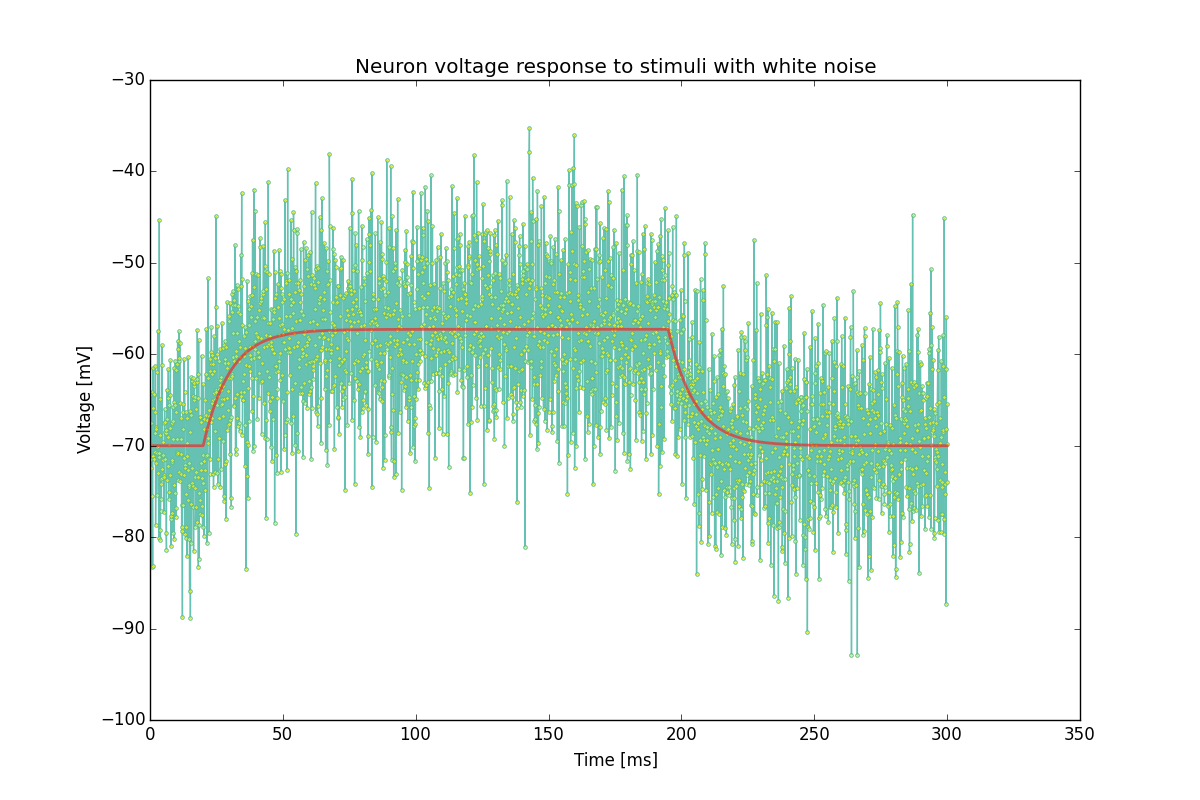
\includegraphics[width=\textwidth]{./fig/noise/white_noise.png}
	\caption[Fehér zaj]{Determinisztikus függvény (piros) és az arra rakott $\sigma_w = 7\left[mV\right]$ szórású fehér zajból előálló szintetikus adatsor (zöld).}
	\label{fig:white}
\end{figure}



\subsubsection{Exponenciálisan korreláló színes zaj}\label{sec:colored_noise}
A kísérleti zajok egy sokkal realisztikusabb modellje az önmagával időben exponenciálisan korreláló színes zaj. Ez a zajmodell jobban leírja az elektrofiziológiai kísérletek során keletkező zajt. 

\paragraph{tulajdonságai}
Tegyük fel hogy a kísérleti zajunk színes zaj $(z=\epsilon)$. Ennek a következő tulajdonságai vannak:
\begin{equation}\label{eq:c1}
\left<\epsilon(t)\right> = 0
\end{equation}
vagyis várható értéke nulla és
\begin{equation}\label{eq:c2}
\left<\epsilon(t)\epsilon(s)\right> = D\lambda \exp\left(-\lambda\left|t-s\right|\right)
\end{equation}
önmagával exponenciálisan korrelál, mivel az autokorrelációs függvénye exponenciálisan lecsengő. Ebben a képletben $D$ az amplitúdó és $\lambda$ pedig a karakterisztikus idő reciproka ($1/\tau$), azt mondja meg, hogy milyen gyorsan cseng le a korreláció időben, az adatpontok között. Szórása a \ref{eq:c1} és \ref{eq:c2} összefüggésekből:

\begin{gather}
	\left<\epsilon(t)\epsilon(t)\right> = \left<\epsilon(t)^2\right> = D\lambda \\
	\left<\epsilon(t)^2\right> - \left<\epsilon(t)\right>^2 = D\lambda \\
	\sigma_\epsilon = \sqrt{D\lambda}
\end{gather}

\paragraph{kovariancia mátrixa}
A színes zaj tulajdonságait visszahelyettesítve a \ref{eq:cov} képletbe, a kovarianciamátrix elemei így alakulnak:
\begin{equation}\label{eq:covmat_col}
\Sigma_{ij} = D\lambda e^{- \lambda |t_i - t_j|} = \sigma_\epsilon^2 e^{- \lambda |t_i - t_j|}
\end{equation}
ahol $t_i$ az $i$-edik időpillanat. Erről az olvasható le, hogy a mátrix diagonálisában ismét a szórás négyzetek helyezkednek el, mivel $e^0=1$. Viszont most az \textit{"offdiagonális"} helyeken is megjelennek a szórásnégyzetek, méghozzá egy ($\tau$) karakterisztikus idővel lecsengő exponenciális szorzótényezővel, ami a diagonálistól távolodva egyre inkább \textit{"kioltja"} az elemeket. Ha $\lambda \rightarrow \infty$, illetve $\tau \rightarrow 0$, akkor visszakapjuk a független, fehér zaj esetét, amikor csak a diagonális elemek nem nullák.


\paragraph{előállítása}
Egy ilyen tulajdonságú zaj előállítása nem triviális feladat. Ronald F. Fox és Ian R. Gatland által kifejlesztett metódust \cite{PhysRevA.38.5938} implementáltuk \textit{Pythonban}.
A \ref{fig:colored}-ábrán látható, hogy hogyan viselkedik egy színes zaj -- jelen esetben az exponenciálisan korreláló. Látható módon ez tényleg korrelál önmagával. Ez a zaj $D = 30$ és $\lambda = 0.1$ paraméterekkel állt elő.


\begin{figure}[h!]
	\centering
	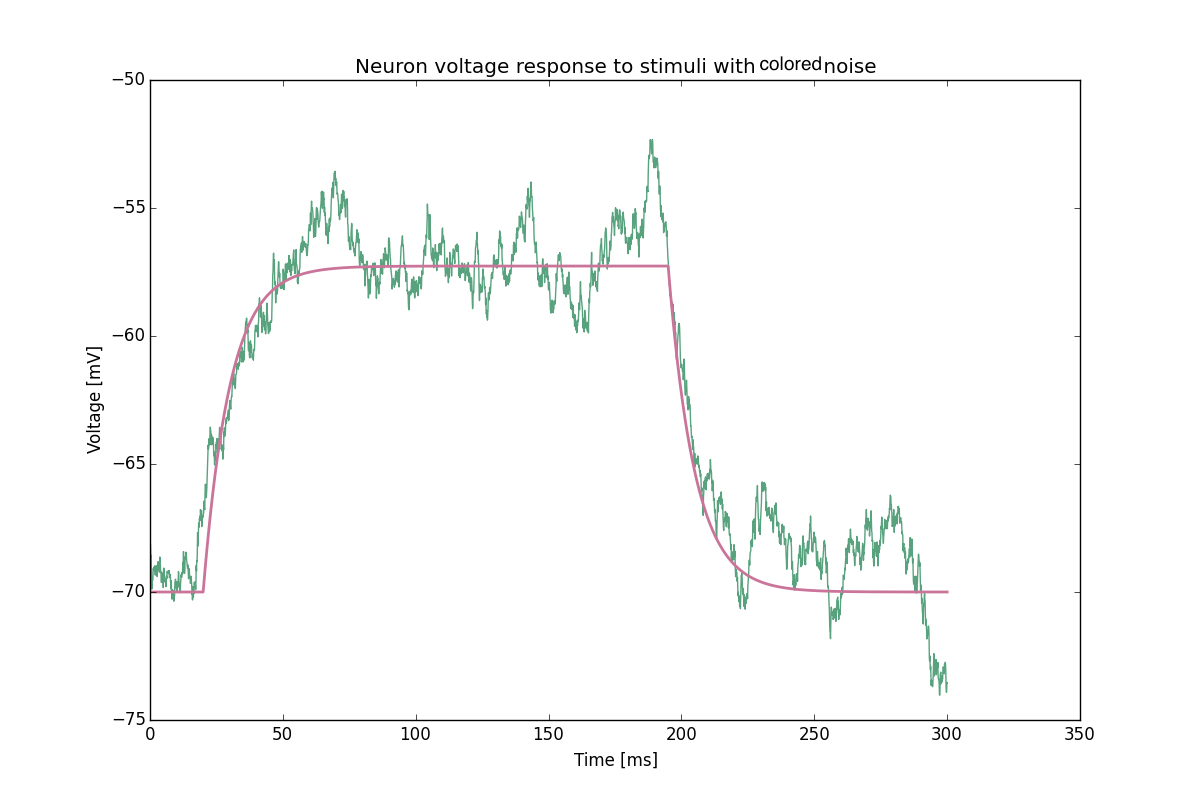
\includegraphics[width=\textwidth]{./fig/noise/colored_noise.png}
	\caption[Színes zaj]{Exponenciálisan lecsengő $\sigma_\epsilon = \sqrt{3} \left[mV\right]$ szórású és $\tau = 10[ms]$ karakterisztikus idejű, exponenciális lecsengésű színes zaj, ami rárakódott a determinisztikus (piros) függvényre, így állítva elő szintetikus adatot. Passzív idegsejt áramimpulzusra adott feszültségválasza jelenik meg a képen. Szemmel látható az időbeli korreláció: az adatpontok fel, illetve lekúsznak szinte folytonosan, nem úgy, mint fehér zajnál.}%
	\label{fig:colored}
\end{figure}




\subsection{Likelihood függvény}\label{sec:likelihood}
A  \ref{sec:bayes} fejezetben már volt szó a likelihood függvény szerepéről. Most arról lesz szó, hogy milyen módszerrel konstruálhatjuk meg.

Azt szeretnénk elérni, hogy a kísérleti adatokat összemérjük a modellünk eredményeivel, a zaj figyelembevétele mellett. Ehhez megvan a modellünk a \textit{Neuron} programban és tegyük fel, hogy kísérleti adataink is vannak. Össze kell hasonlítanunk a kísérleti eredményünket a modell szolgáltatta eredménnyel. Az eltérést látható például a \ref{fig:colored}-ábrán is, ahol a zölddel jelöljük a kísérleti adatokat és a piros (determinisztikus) függvény a modellünk -- adott paraméterek melletti -- eredménye.

Ezekhez a paraméterekhez  -- melyek a \ref{fig:colored} vagy \ref{fig:white} ábrákon a piros függvénymenetet eredményezték -- szeretnénk egy valószínűségi értéket társítani, ami jellemzi a kísérleti adatokkal való egybevágóságot. Legáltalánosabb módszer az adatpontok négyzetes eltéréseit venni és ezzel jellemezni a két függvénymenet \textit{"távolságát"}. A likelihood függvényünket úgy konstruáltuk meg, hogy az így kapott eltérésnégyzeteket beleraktuk egy -- kísérleti zajnak megfelelő szórású -- normál eloszlásba. Következő pontokban megnézzük a likelihood jelentését, valamint matematikai formába öntjük.

\subsubsection{Likelihood értelmezése}
A likelihood függvény tulajdonképpen úgy áll elő, hogy a kísérleti adatsorom ($D$) és a modellem ($\M$) -- adott paraméterek melletti ($\Theta$) -- eredményének különbségét berakom a zaj eloszlásfüggvényébe ($P_z$), amely esetünkben egy megfelelő szórású -- vagy kovariancia mátrixú -- normál eloszlás lesz ($\N$):
\begin{equation}
\Lagr\left(D|\Theta\right) = P_z\left(D-\M\left(\Theta\right)\right) = \N\left(D-\M\left(\Theta\right)\right)
\end{equation} 

Másképp megfogalmazva a likelihood megmondja, hogy az adott paraméterek melletti determinisztikus modelleredményt kivonva az adatsorból, milyen mértékben kapjuk vissza a zajt:
\begin{gather}
	D = D^* + z = \M\left(\Theta^*\right) + z \\
	\Lagr\left(D|\Theta\right) = P_z\left(z + \M\left(\Theta^*\right) -\M\left(\Theta\right)\right)
\end{gather}

\subsubsection{Normál eloszlásból likelihood}
A függvény alakjának tehát célszerű a normál (Gauss) eloszlást választani, amely egydimenziós esetében az alábbi módon néz ki:

\begin{equation}\label{eq:gauss}
	\N\left(x|\mu, \sigma^2\right) = \dfrac{1}{\sqrt{2\pi \sigma^2}}e^{-\dfrac{\left(x-\mu\right)^2}{2\sigma^2}}
\end{equation}
ahol $\mu$ a valószínűségi változó várható értéke és $\sigma$ pedig a szórása.

A likelihood függvényünket ebben a formában szeretnénk kifejezni, ehhez a következőket kell tennünk fehér zaj esetén: vesszük az adatpontok négyzetes eltéréseinek összegét $\left(\sum_{i=1}^{N}x_i^2\right)$, melyet jelöljük $x_s(D,\Theta)^2$-el -- mely a modell aktuális paramétereinek értékektől és a kísérleti adatoktól függ --, valamint a zaj szórása legyen $\sigma_w$. Ekkor a likelihood függvényünk az alábbi alakú lesz:
\begin{equation}\label{eq:likelihood}
	\Lagr\left(D|\Theta\right)  \propto e^{-\dfrac{x_s^2}{2\sigma_w}}
\end{equation}
Elég arányosságról beszélni, mivel a végén úgyis normáljuk az eredményünket.


Mivel a kísérleti adatsorunk sok pontból áll és színes zaj esetén ezek az adatpontok nem függetlenek, érdemes az általános $N$ dimenziós normál eloszlást bevezetni:
\begin{equation}\label{eq:gaussD}
	\N\left(\gv{x}|\gv{\mu}, \underline{\underline{ \Sigma }}\right) = \dfrac{1}{\sqrt{\left(2\pi\right)^{D} \det \underline{\underline{ \Sigma }}}}\exp\left[-\dfrac{1}{2}\left(\gv{x}-\gv{\mu}\right)^T \underline{\underline{ \Sigma }}^{-1}\left(\gv{x}-\gv{\mu}\right)\right]
\end{equation}
ahol $\underline{\underline{ \Sigma }}$ a valószínűségi változók kovariancia mátrixa, $\gv{\mu}$ pedig a hozzájuk tartozó várható érték.


Az általános likelihood függvényünk ezek alapján a következő módon áll elő:
\begin{equation}\label{eq:likelihoodN}
	\Lagr(D|\Theta) \propto \exp\left[-\dfrac{1}{2}\gv{x}^T \underline{\underline{ \Sigma }}^{-1}\gv{x}\right]
\end{equation}
ahol $\gv{x}(D,\Theta)$ a modell determinisztikus eredményének ($\M\left(\Theta\right)$) és a kísérleti adatsornak ($D$) az eltérésvektora\footnote{Ami tulajdonképpen nem más mint a zaj, a megfelelő paraméterek esetén, azaz: $\left(D-\M\left(\Theta^*\right)\right) = z$}. Minden $t$ mérési időponthoz egy érték tartozik, tehát a vektor annyi elemből áll, ahány mérési pontunk van. A fenti képletben $\underline{\underline{ \Sigma }}$ pedig a zaj kovariancia mátrixa.

\paragraph{független eset}
Speciális eset ha a kovariancia mátrixnak csak a főátlójában helyezkednek el tagok, ami azt jelenti, hogy a pontok függetlenek (a zaj időben független), így szétválik a valószínűségi eloszlásfüggvény az egydimenziós esetek szorzat alakjára. Ha feltesszük, hogy a diagonálisban ráadásul ugyan azok a szórásértékek szerepelnek, akkor:

\begin{equation}\label{eq:likelihoodN_independent}
\exp\left[-\dfrac{1}{2}\gv{x}^T \underline{\underline{ \Sigma }}^{-1}\gv{x}\right] \rightarrow 	 e^{-\dfrac{x_s^2}{2\sigma_w}}
\end{equation}
Tehát az általános -- nem feltétlenül független -- esetből visszakaptuk a független esetet.


\subsubsection{Likelihood megkonstruálása numerikusan}
Tekintsük át a lépéseket, melyekkel előállítjuk a likelihood függvényünk. A \ref{eq:likelihoodN} képletnek kell szolgáltatni egy $\gv{x}$ vektort és egy $\underline{\underline{\Sigma}}$ mátrixot, amely végül eredményül egy skalárt ad, ami az adott paraméterkombináció \textit{"jóságát"} jellemzi. Az előbbi a pontbeli eltérésekből gyártott vektor $\left(D-\M\left(\Theta\right)\right)$, az utóbbi pedig a kísérletből fakadó zaj autokorrelációs függvénye által meghatározott kovariancia mátrix.

Ha az adatpontokat függetleneknek, vagy függőknek tekintjük, érdemes különböző módon eljárni, mivel független esetben olyan egyszerűsítések végezhetők, melyek csökkentik a számítás és memóriaigényt:
 
 \paragraph{független eset}
Ebben az esetben azért végezhetők egyszerűsítések, mert a valószínűségi változók függetlennek, így az eloszlásfüggvény sokdimenziós alakból egydimenziós eloszlások szorzataira bomlik. Ekkor a likelihood értékek konstruálását a következő lépések írják le:
\begin{enumerate}\label{meth:independet}
	\item Adott paraméterkombinációval ($\gv{\Theta}_i$) lefuttatjuk a szimulációt ($\M$) a \textit{NEURON} program segítségével.
	\item Megnézzük a kísérleti és a szimulációs adatok négyzetes eltérését minden ($N$) pontban ($x_j^2$) és összegzünk is erre ($x_s^2 = \sum_{j=1}^{N} x_j^2$).
	\item Az összegzett értéket megszorozzuk $-1/(2 \sigma_w^2)$ -tel, ahol $\sigma_w$ a független zaj szórása.
	\item Ezt elvégezzük az összes lehetséges paraméterkombinációra ($\forall i$) és tároljuk az eredményeket. Numerikus okokból érdemes a legnagyobb értéket kivonni az összesből\footnote{Ezzel nem változtatunk semmit az eredményen, mivel csak eltoljuk a függvényt -- ami negatív értékkészletű --  úgy, hogy maximuma a nullába kerüljön -- így a maximális likelihood értékhez $e^0 = 1$ társul majd --, de az alakja nem változik. A transzformáció segítségével viszont elérjük, hogy ne kelljen túl kicsi számokkal dolgozni, ami numerikusan problémákhoz vezethet.}.
	\item Végül ezt exponencializálva megkapjuk az egyes paraméterkombinációkhoz tartozó likelihood értéket: $ \Lagr_i(D|\gv{\Theta}_i)$, ahol $i$ végigfut az összes lehetséges paraméterkombináción.
\end{enumerate}

\paragraph{átalános eset}
Általános nem független esetben az előző lépések így módosulnak:
\begin{enumerate}\label{meth:dependet}
	\item Adott paraméterkombinációval ($\gv{\Theta}_i$) lefuttatjuk a szimulációt ($\M$) a \textit{NEURON} program segítségével.
	\item Megnézzük a kísérleti és a szimulációs adatok eltérését minden pontban és ezeket egy vektorban tároljuk: $\gv{x} = D-\M\left(\gv{\Theta}_i\right)$.
	\item A zaj inverz kovariancia mátrixát megszorozzuk balról és jobbról is az előbbi különbségvektorral és ezt egy további $-1/2$ faktorral: $-1/2\cdot\gv{x}^T\underline{\underline{\Sigma}}^{-1}\gv{x}$
	\item Ezt elvégezzük az összes lehetséges paraméterkombinációra ($\forall i$) és tároljuk az eredményt. Numerikus okokból érdemes a legnagyobb értéket kivonni az összesből.
	\item Végül ezt exponencializálva megkapjuk az egyes paraméterkombinációkhoz tartozó likelihood értéket: $ \Lagr_i(D|\gv{\Theta}_i)$, ahol $i$ végigfut az összes lehetséges paraméterkombináción.
\end{enumerate}

\paragraph{poszterior megalkotása}
Ezután mindkét esetben hasonlóan járunk el: a likelihood függvény elemeit összeszorozzuk a prior eloszlás megfelelő elemeivel: $\mathcal{Z}_i=\Lagr_i(D|\gv{\Theta}_i)\Pi_i\left(\gv{\Theta}_i\right)$. Végezetül ezt normálva kapjuk meg a poszterior eloszlásunkat: $P\left(D|\Theta\right) = \mathcal{Z}/\left(\sum_{i}\mathcal{Z}_i\right)$. Ezzel egy Gauss-görbére emlékeztető alakú poszterior eloszlást kapunk végeredményként, a vizsgált paramétertartomány fölött, amely a kísérlet és az előzetes ismeretek alapján egy valószínűségi értéket rendel az egyes paraméterkombinációkhoz.

Azt hogy az adatpontok milyen módon függnek és ekkor mi lesz a \ref{eq:likelihoodN} likelihood függvényben szereplő kovariancia mátrix, a kísérleti zaj határozza meg. Ha a kísérletből nem származna zaj (\ref{sec:noise}-ben $D = D^*$, tehát $z=0$), ekkor a kísérleti adatok determinisztikusak lennének és ennek a dolgozatnak nem lenne feladata -- függetlenek lennének az adatpontok nulla szórással -- és egyszerű paraméteroptimalizációs algoritmus elegendő lenne a tökéletes paraméterek megtalálásához, feltéve hogy maga a modell is tökéletes. Tehát ekkor már csak az lenne a kérdés, hogy a modell mennyire jól írja le a valóságot.

Az inferencia eredményeinek tipikus ábrázolási módjaira láthatunk példát a \ref{fig:marginal_joint} és \ref{fig:fullplot}-ábrákon.

\begin{figure}[h!]
	\centering
	\subfloat[Marginális eloszlás]{{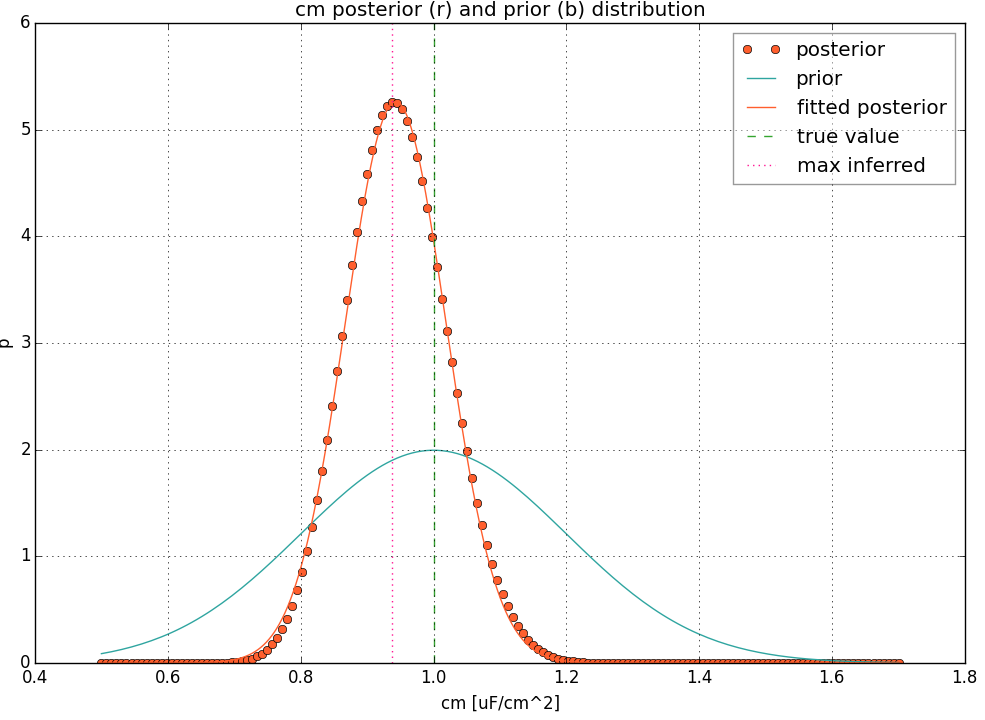
\includegraphics[width=0.4\textwidth]{./fig/figtypes/cm_P(10).png} }}
	\subfloat[Együttes eloszlás]{{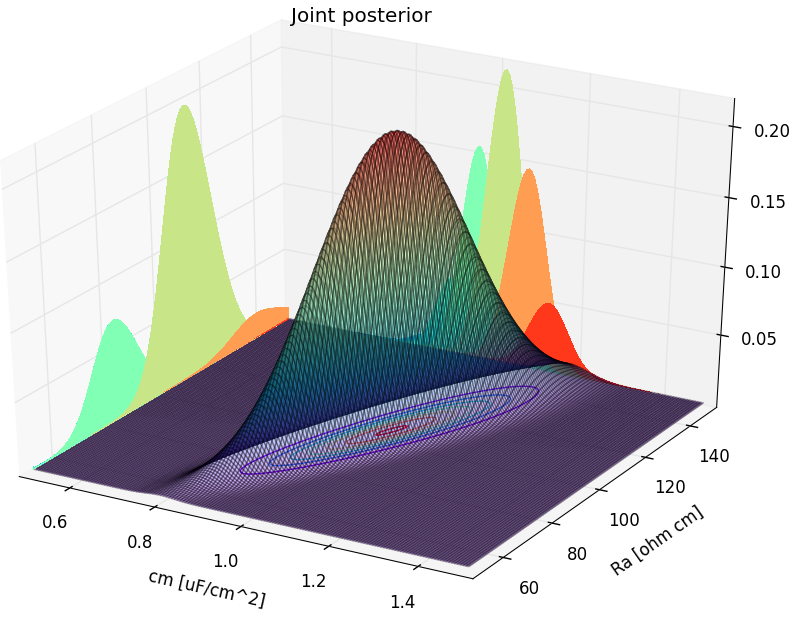
\includegraphics[width=0.4\textwidth]{./fig/figtypes/P_Ra-cm(7).png} }}%
	\caption[Marginális eloszlás és együttes eloszlás típikus ábrái]{Egy paraméterre vett marginális eloszlás egy tipikus ábrázolása látható az (a) ábrán. Kékkel a prior eloszlás, narancssárgával pedig az inferencia után kapott poszterior eloszlás. A szaggatott zöld vonal jelzi azt a paramétert, amelyet a szintetikus adat előállításánál használtunk. Pontozott piros vonal jelöli a paraméterbecslésünk által talált legvalószínűbb értéket. A (b) ábrán pedig két paraméter eloszlásának egy tipikus ábrája. Az egyes síkokra a kontúrvonalak vannak levetítve.}%
	\label{fig:marginal_joint}
\end{figure}


\begin{figure}[h!]
	\centering
	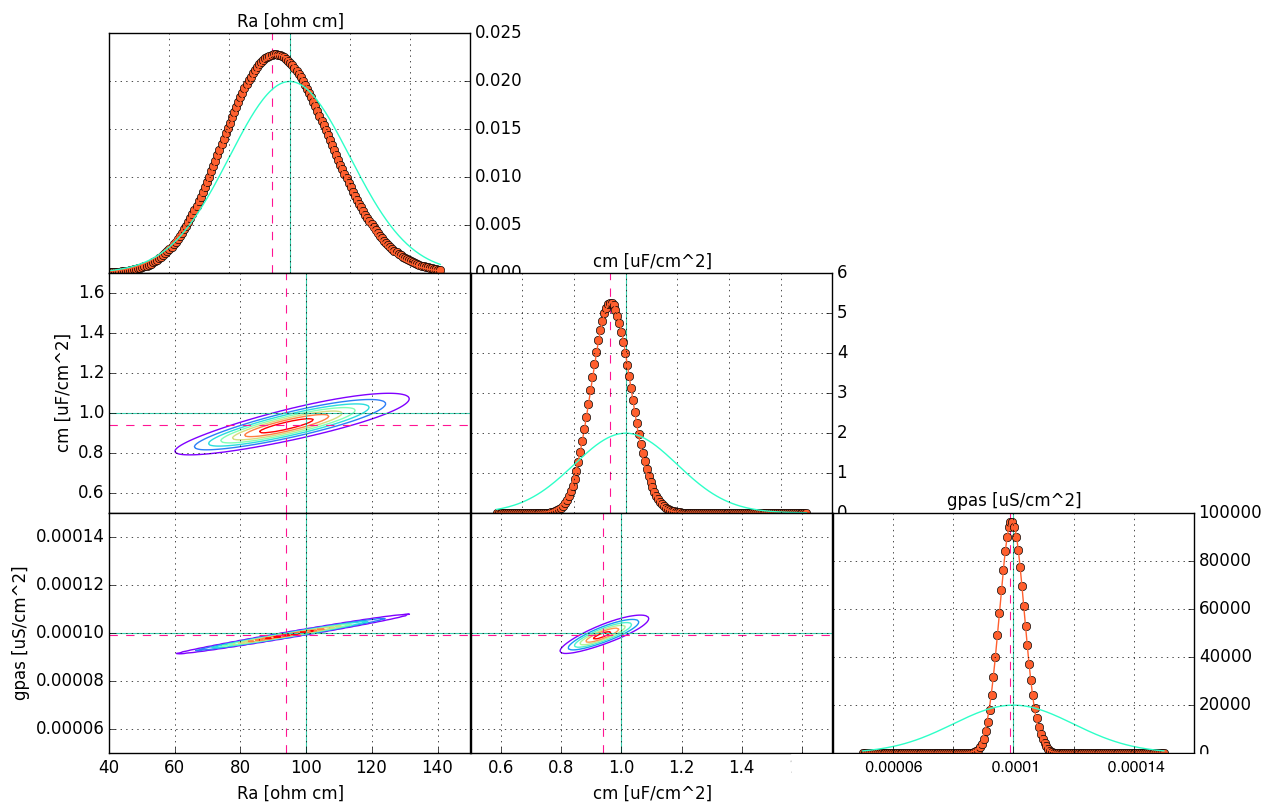
\includegraphics[width=\textwidth]{./fig/figtypes/fullplot_P(10).png}
	\caption[Együttes és marginális eloszlásokat összefoglaló ábratípus]{Sok paraméter esetén -- jelen esetben három -- már csak több ábra együttesével vagyunk képesek jellemezni az eredményt. Ezen az ábrán három paraméter marginális és együttes eloszlásai vannak feltüntetve, megfelelő sorrendben. A \textit{"diagonálisban"} láthatóak az egyes paraméterek marginális poszterior (narancs) és prior (kék) eloszlásai, alattuk/mellettük pedig rendre a paraméterek együttes levetített kontúr eloszlásai. Kék vonallal vannak jelölve azok a paraméterértékek, melyekből generáltuk a szintetikus adatot és magenta színű szaggatott vonallal pedig az inferencia által maximálisnak becsült értékek.}%
	\label{fig:fullplot}
\end{figure}

\subsection{Technikai megvalósítás}
A program \textit{Pythonban} lett írva, modern, moduláris megvalósítással, így segítségével gyorsan és egyszerűen össze lehet állítani különböző futtatási modelleket. A szimulációk kiértékelése párhuzamosítva történik, így egyszerre több processzormagon is folynak a számítások, hogy a teljes erőforrás ki legyen használva. A forráskód verziókövetve lett a \textit{GitHubon}, ez a következő link alatt érhető el: \url{https://github.com/terbed/parameter-inference}. Lineáris algebrai számításokhoz, az erre a célra kifejlesztett és hatékony \textit{NumPy} csomagot alkalmaztuk, vizualizációhoz pedig a \textit{Matplotlib}et.

Egy paraméterbecslés összeállításának tipikus menete, azaz egy példakód látható a \ref{fig:code}-ábrán és magyarázat az ábraleírásban. Először a különböző paramétereket kell beállítani, majd ezeket sorjában megadni a \textit{ParameterSet} objektumnak, amely elkészíti a paramétertér felosztását. Ez bármennyi paraméterre, általánosan működik. Viszont a paraméterek számának növekedésével robbanásszerűen nő a futtatandó szimulációk száma is, így a \textit{"brute force"} megoldás, vagyis az egész paramétertér kiértékelése gyakorlatilag nem fut le ésszerű időn belül -- bizonyos számú paraméter és felbontás mellett. Következő lépésben a \textit{ParameterSet} objektumot meg kell adni az inferenciát végző, a példa esetében \textit{IndependentInference} objektumnak, amely ezen kívül még vár zajszórást, céladatsort és szimulációs modellt. Inicializálás után az osztály \textit{run\_sim()} metódusával kezdjük el kiértékelést több szálon is. Végül az eredmények vizualizációja is automatikusan történik.

\begin{figure}[h!]
	\centering
	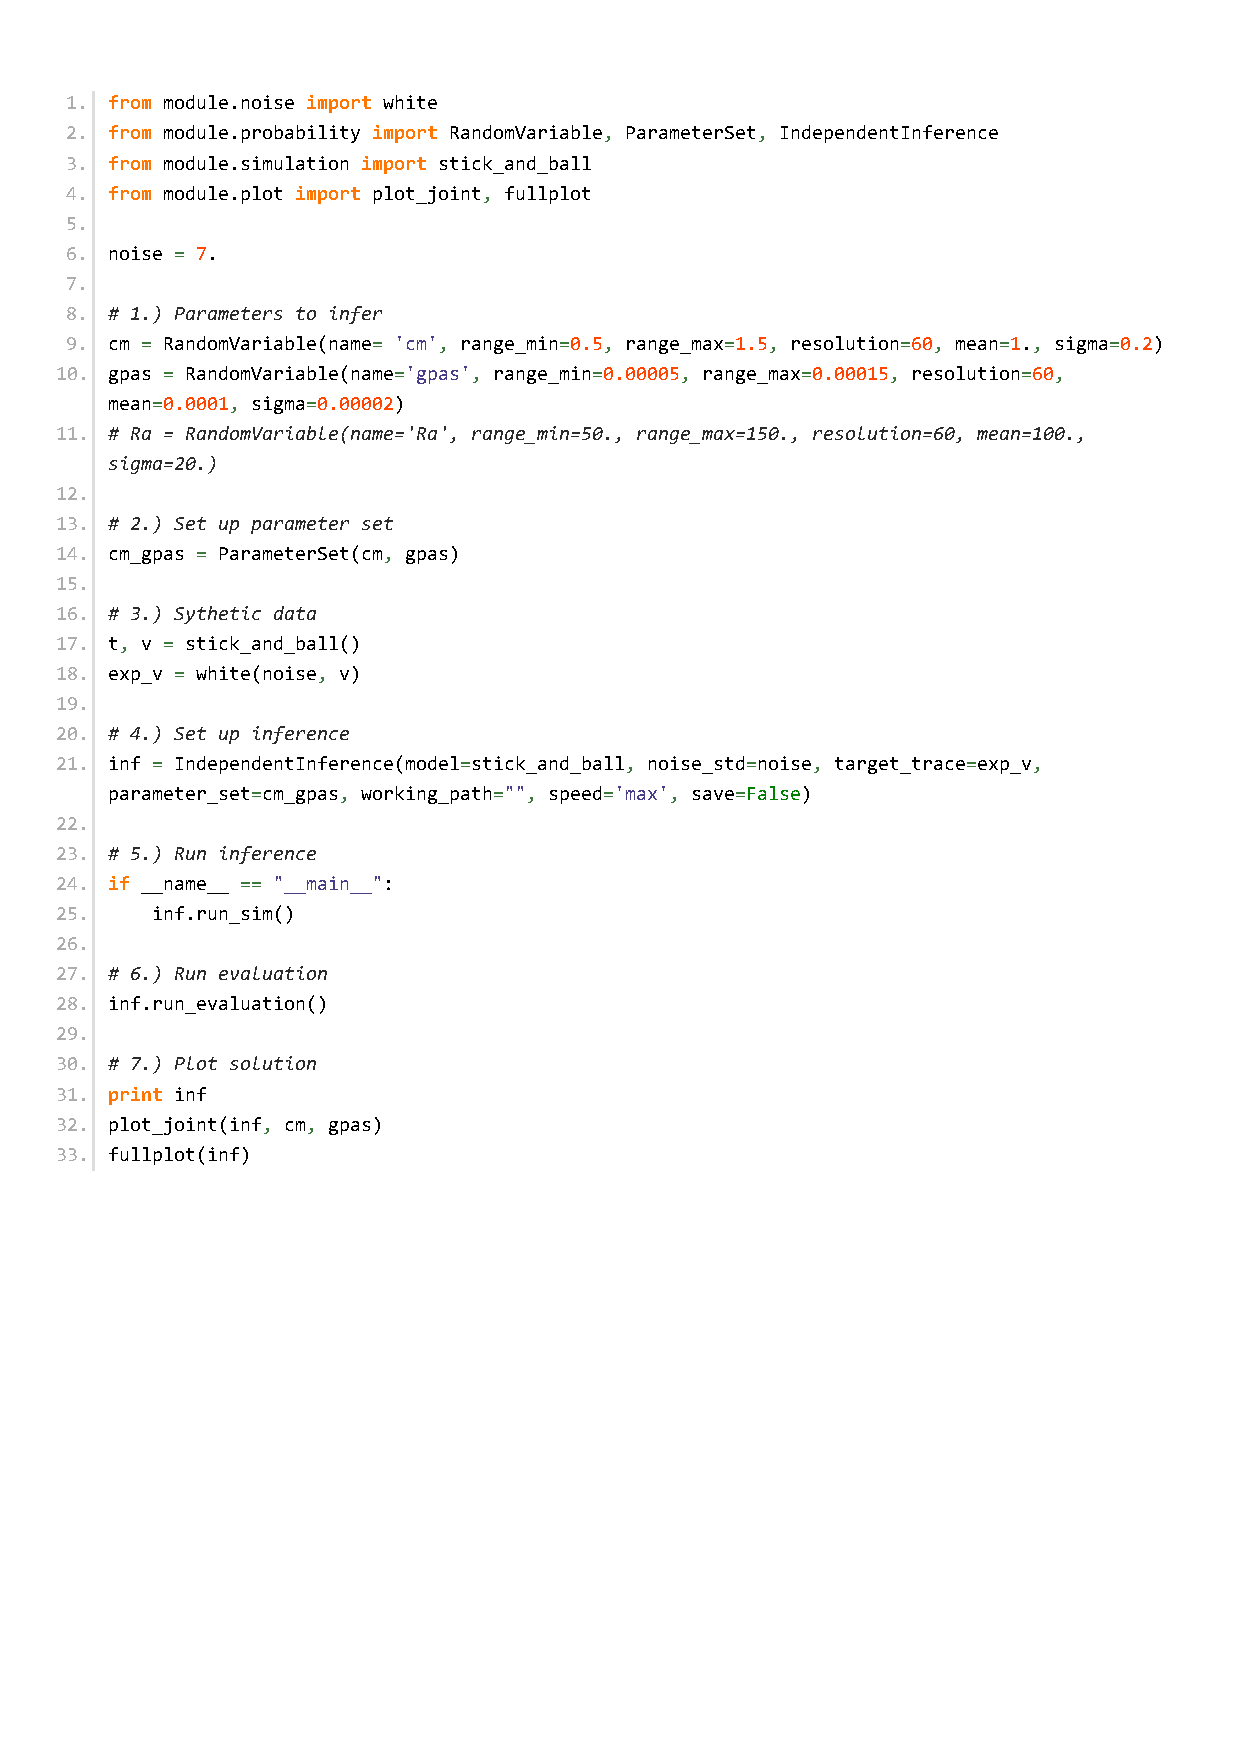
\includegraphics[width=\textwidth]{./fig/source.pdf}
	\caption[Egy futtatás példakódja]{Egy kétparaméteres, fehér zajos \textit{Stick and Ball} modell inferenciája látható. Az importált modulok rövid leírása: A \textit{noise} modul tartalmazza a fehér és színes zaj generálásához szükséges kódot. A \textit{probability} modul az inferencia lelke, itt történik az egyes paraméterek és a paraméterkombinációk (paramétertér) létrehozása, valamint a kiértékelésük is. A \textit{simulation}ben találhatóak az épített idegsejtmodelljeink, itt történik az interakció a \textit{NEURON} programmal. A \textit{plot} modulban találhatók a vizualizációért felelős kódok.}
	\label{fig:code}
\end{figure}

\FloatBarrier
\subsection{Összegzés}
Az előző pontokban láttuk, hogyan hozhatunk létre zajmodelleket és likelihood függvényt, majd abból poszterior eloszlást. Szintetikus adatok előállításával és azon végzett inferenciával szeretnénk az egyes kísérleti protokollok információtartalmát jellemezni, melyek a vizsgált idegsejt anatómiájából (térbeli kiterjedés), biofizikai tulajdonságaiból (pl. passzív modell, vagy Hodgkin-Huxley aktív modell), ingerlés típusából (stimulus helye és formája), valamint az idegsejten végzett mérés helyéből tevődik össze. A \ref{fig:method}-ábrán látható az előbbiek sematikus rajza.



\begin{figure}[h!]
	\centering
	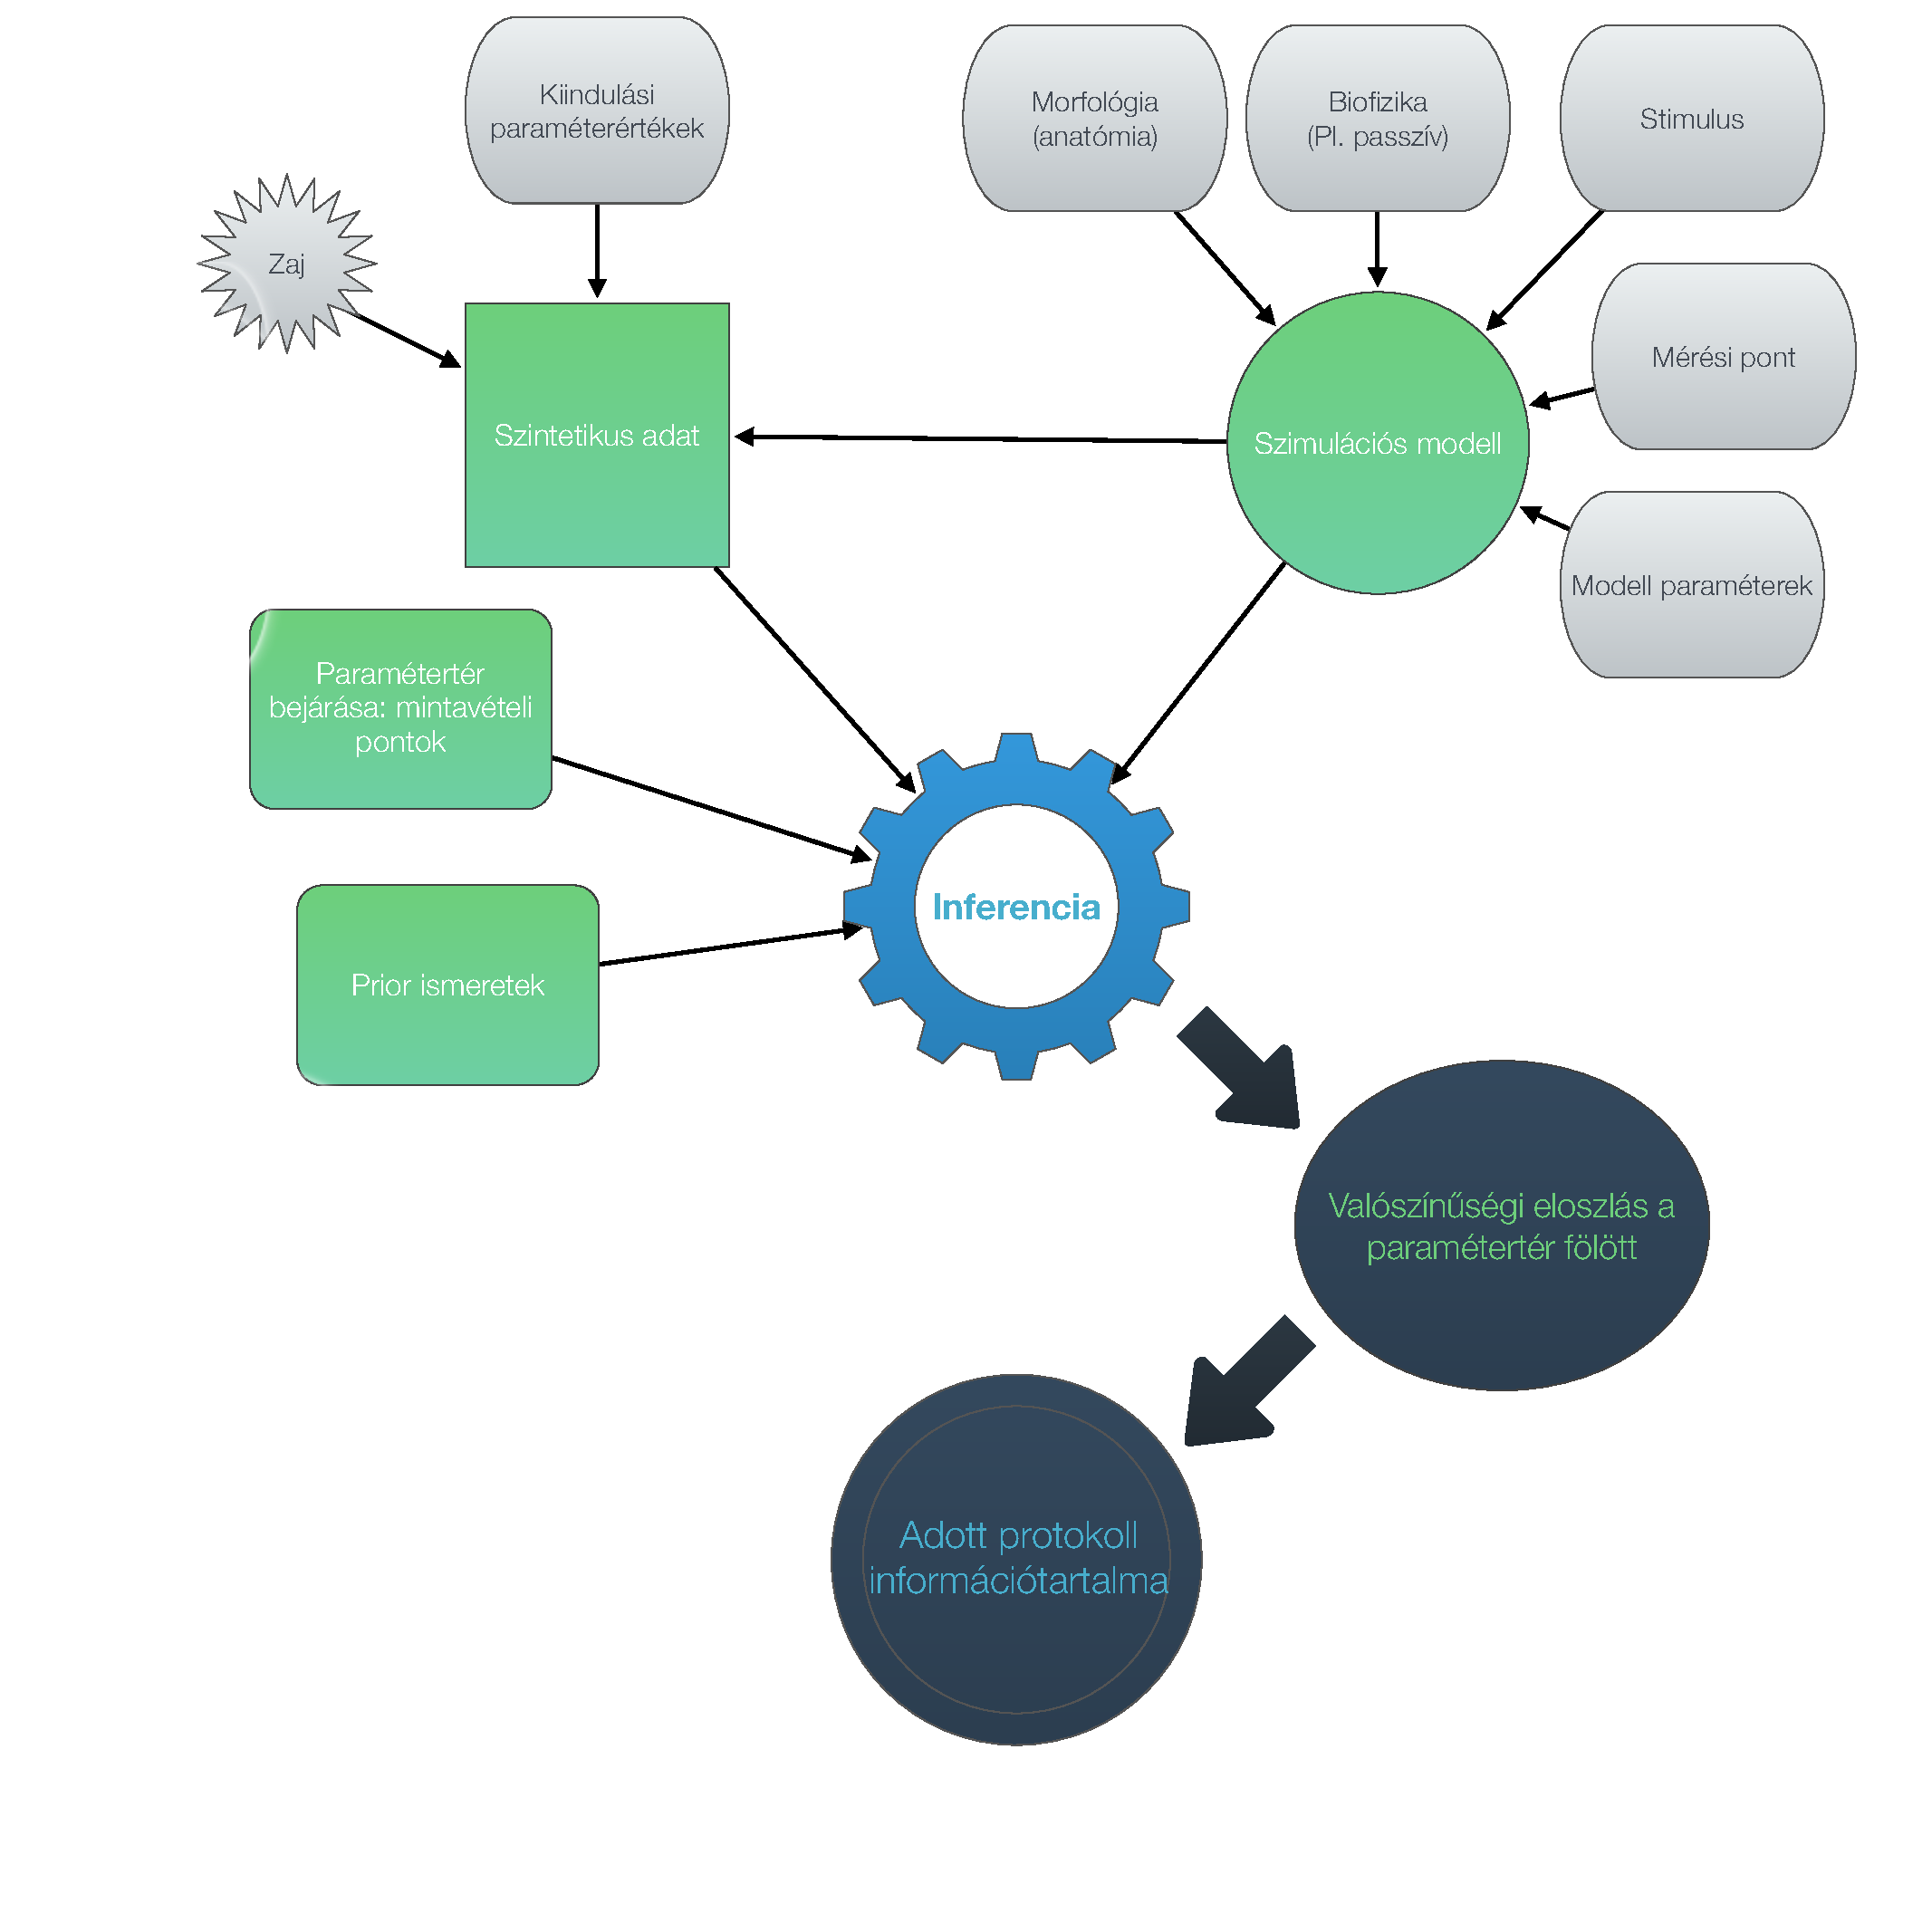
\includegraphics[width=0.6\textwidth]{./fig/method.pdf}
	\caption[Módszer sémája]{Ezen az ábrán a módszer sémája látható.}%
	\label{fig:method}
\end{figure}


